\documentclass[crop,tikz,convert={outext=.svg,command=\unexpanded{pdf2svg \infile\space\outfile}},multi=false]{standalone}[2012/04/13]
%\usetikzlibrary{...}% tikz package already loaded by 'tikz' option

%%% Tikz libraries and definitions
\usetikzlibrary{intersections}
\usetikzlibrary{arrows}
\usetikzlibrary{calc}                 % coordinate calculations ($ n1 + (0:1cm) $)

% Common style for Simulink blocks.
\tikzstyle{block} = [rectangle, rounded corners, minimum width=3cm, minimum height=0.8cm,text centered, thick, draw=black]
% Common style for connectors. 
\tikzstyle{arrow} = [->,>=stealth',font=\scriptsize,rounded corners]

% Some distances to share between figures.
\newcommand{\shift}{0.28cm}
\newcommand{\bigshift}{1cm}

\begin{document}

  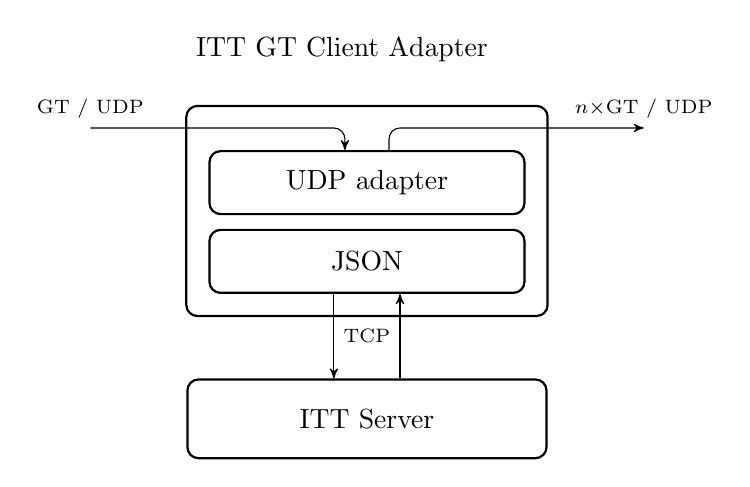
\begin{tikzpicture}[node distance=1.5cm, block/.append style={minimum width=4cm}]
  

  % Inner blocks
  \node [block]                                    (udp) {UDP adapter};

  \node [block, below of=udp, node distance=1.0cm] (json) {JSON};

  %  box
  \draw ([xshift=-\shift, yshift=\shift+\shift]udp.north west) [block] rectangle  ([xshift=\shift,yshift=-\shift]json.south east);  

  %  label
  \node [anchor=south west] (access) at ([xshift=-\shift, yshift=\bigshift]udp.north west) {ITT GT Client Adapter};



  % ITT Server
  \node [block, below of=json, node distance=2.0cm, minimum width=4cm+2*\shift, minimum height=1cm] (tap) {ITT Server};



  % GN - UDP-to-Eth
  \draw [arrow] ([xshift=-1.5*\shift]json.south) node [name=gnLeft] {} -- node [anchor=west] {TCP} (gnLeft |- tap.north);

  \draw [arrow, <-] ([xshift=1.5*\shift]json.south) node [name=gnRight] {} -- (gnRight |- tap.north);



  % In
  \draw [arrow] ([xshift=-1.5*\bigshift,yshift=\shift]udp.north west) node [anchor=south] {GT / UDP} -| ([xshift=-\shift]udp.north);

  % Out
  \draw [arrow, <-] ([xshift=1.5*\bigshift,yshift=\shift]udp.north east) node [anchor=south] {$n \times$GT / UDP} -| ([xshift=\shift]udp.north);

  \end{tikzpicture}

\end{document}